\documentclass[11pt, letterpaper]{article}
\usepackage[utf8]{inputenc}
\usepackage[letterpaper, margin=0.5in]{geometry}
\usepackage{amsmath}
\usepackage{amssymb}
\usepackage{amsthm}
\usepackage{graphicx}
\usepackage{listings}
\usepackage[font=scriptsize]{caption}
\usepackage{subcaption}
\usepackage{xcolor}

\definecolor{codegreen}{rgb}{0,0.6,0}
\definecolor{codegray}{rgb}{0.5,0.5,0.5}
\definecolor{codepurple}{rgb}{0.58,0,0.82}
\definecolor{backcolour}{rgb}{0.95,0.95,0.92}

\lstdefinestyle{mystyle}{
    backgroundcolor=\color{backcolour},   
    commentstyle=\color{codegreen},
    keywordstyle=\color{magenta},
    numberstyle=\tiny\color{codegray},
    stringstyle=\color{codepurple},
    basicstyle=\ttfamily\footnotesize,
    breakatwhitespace=false,
    texcl=true,
    mathescape=true,
    breaklines=true,                 
    captionpos=b,                    
    keepspaces=true,                 
    numbers=left,                    
    numbersep=5pt,                  
    showspaces=false,                
    showstringspaces=false,
    showtabs=false,                  
    tabsize=2
}

\lstset{style=mystyle}
\graphicspath{ {.} }
\captionsetup{justification=raggedright, singlelinecheck=false}

\author{Ryan Tang}
\title{STA 602 HW 11}
\date{November 18th 2022}

\begin{document}
\maketitle

\section{Exercise 9.1}
\paragraph{(a) Analysis}
We have the following graphical model, one for each swimmer $k \in \{1, \dots, K=4\}$. For each swimmer, we have worth of 6 weeks of data points that records their swim time for a 50 yards run, $i \in \{1, \dots, N=6\}$. Here we like to fit a linear regression for each swimmer; thus, in total of 4 linear regression, each with its respective priors.
\begin{figure*}[!h]
  \centering
  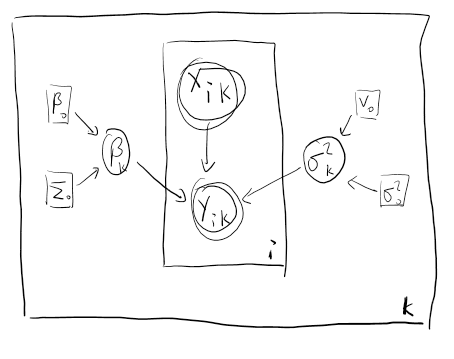
\includegraphics[width=0.4\textwidth]{1.2.graph.png}
  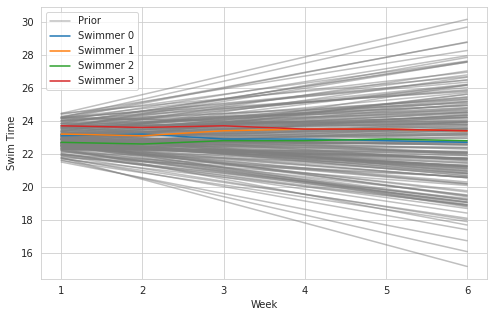
\includegraphics[width=0.45\textwidth]{1.1.png}
  % \captionsetup{justification=centering}
  \caption{(Left) Typical Bayesian Linear Regression Graphical Model. (Right) Prior Believe Check. Each grey line is a sampled prediction using just the priors.}
  \label{fig:ex9.1_model}
\end{figure*}

We are also given some knowledge on typical competitive times for the age group range from 22 to 24 seconds. We will use this to construct out priors accordingly, and the following is the full spec of the model. Some notations, $X_{k} \in \mathbf{R}^{N\times p}$, $\bold{y}_k \in \mathbf{R}^N$, and $\beta_k \in \mathbf{R}^p$, where $p = 2$ in our case, one for the intercept, and one for the weeks.
\begin{align*}
    y_{ik} &\mathop{\thicksim}^{iid} \mathcal{N}(X_k \beta_k, \sigma_k^2 \mathbf{I}_n) \\
    \beta_k &\thicksim \mathcal{N}(\beta_o, \Sigma_o) \\
    1/\sigma^2_k = \gamma_k &\thicksim \text{Gamma}(\frac{\nu_o}{2}, \frac{\nu_o\sigma^2_o}{2})
\end{align*}
Here we specified $\beta_o = (23, 0)^{\intercal}$, $\Sigma_o = \begin{bmatrix}0.2 & 0 \\ 0 & 0.2\end{bmatrix}$, $\nu_0 = 1$, $\sigma^2_o = 1$, and the resulting prior believes is also plotted in Figure \ref{fig:ex9.1_model}, right plot.

\newpage
Lastly, we obtained the posterior predictive distribution using the resulting linear regression assuming all swimmers had only swim two weeks from the last recorded time. The distributions are plotted in Figure \ref{fig:ex9.1_pp}
\begin{figure}[!h]
  \centering
  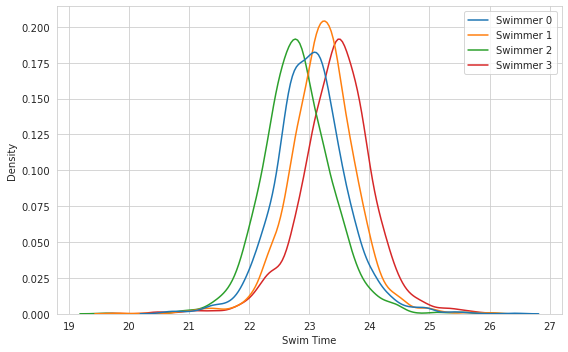
\includegraphics[width=0.45\textwidth]{1.3.png}
  \captionsetup{justification=centering}
  \caption{Posterior predictive distribution of Swim Time given only swim two weeks from the last recorded time.}
  \label{fig:ex9.1_pp}
\end{figure}

\paragraph{(b) Recommendation}
In order to make a recommendation to the coach, we took the posterior predictive samples and calculated $Pr(Y_j^* = max\{Y_k\}|Y)$. We already have the samples while constructing the Figure \ref{fig:ex9.1_pp}. Hence, the resulting probability bar chart is shown in Figure \ref{fig:ex9.1_pp_pr_max}. According to the analysis, we should consider swimmer 3.
\begin{figure}[!h]
  \centering
  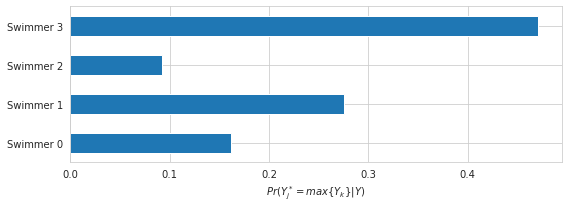
\includegraphics[width=0.65\textwidth]{1.4.png}
  \captionsetup{justification=centering}
  \caption{Probability for being the best.}
  \label{fig:ex9.1_pp_pr_max}
\end{figure}


\newpage
\section{Exercise 9.2}
We are revisiting the diabetes dataset, with a interest of doing inference on the glucose level. We used all other covariates, except `diabetes`, in the training of the Bayesian linear regression model. Hence the design matrix $X \in \mathbf{R}^{N\times (p+1)}$, where $N = 532$ and $p = 6$.

\paragraph{(a) Linear Regression}
First, we fit a typical regression using all covariates and a g-prior for $\beta$. Therefore, we have the following model specs.
\begin{align*}
    y_i &\thicksim \mathcal{N}(X\beta, \sigma^2) \\
    1/\sigma^2 = \gamma &\thicksim \text{Gamma}(\frac{\nu_o}{2}, \frac{\nu_o\sigma_o^2}{2}) \\
    \beta &\thicksim \mathcal{N}(0, g\sigma^2(X^{\intercal}X)^{-1})
\end{align*}
We set $\nu_o = 2$, $\sigma^2_o = 1$ and $g = n = 532$. The resulting confidence interval of all parameters are shown in the below table.

\begin{center}
\begin{tabular}{||c|c c c c c c c c||}
\hline
95\% CI & $\beta$ intercept & $\beta$ npreg & $\beta$ bp & $\beta$ skin & $\beta$ bmi & $\beta$ ped & $\beta$ age & $\sigma^2$ \\
\hline\hline
2.5\% & 35.12 & -1.62 &	-0.035 & -0.11 & 0.15 & 2.98 & 0.44 & 746.87 \\ 
97.5\% & 70.04 & 0.30 & 0.43 & 0.51 & 1.16 & 17.94 & 1.08 & 937.10 \\
\hline
\end{tabular}
\end{center}

\paragraph{Bayesian Model Selection and Averaging (BMA)}
Here we like to do BMA and the simplest way we can perform this is by assigning a binary vector $\bold{z} \in \mathbb{R}^p$ the same size of $\beta$, with each $z_j$ be a independent Bernoulli random variable. Hence, the resulting model becomes as the following. Note, $\circ$ is the Hadamard product.
\begin{align*}
    y_i &\thicksim \mathcal{N}(X(\bold{z} \circ \beta), \sigma^2) \\
    z_j &\thicksim \text{Bernoulli}(q) \\
    1/\sigma^2 = \gamma &\thicksim \text{Gamma}(\frac{\nu_o}{2}, \frac{\nu_o\sigma_o^2}{2}) \\
    \beta &\thicksim \mathcal{N}(0, g\sigma^2(X^{\intercal}X)^{-1})
\end{align*}

\begin{center}
\begin{tabular}{||c|c c c c c c c c||}
\hline
95\% CI & $\beta$ intercept & $\beta$ npreg & $\beta$ bp & $\beta$ skin & $\beta$ bmi & $\beta$ ped & $\beta$ age & $\sigma^2$ \\
\hline\hline
2.5\% & 53.81 & -0.86 & 0.0 & 0.0 & 0.76 & 0.0 & 0.59 & 760.39 \\ 
97.5\% & 74.09 & 0.0 & 0.0 & 0.0 & 1.25 & 14.18 & 0.91 & 916.90 \\
\hline
\end{tabular}
\end{center}




\section{Exercise 9.3}


\end{document}